Nos últimos anos, e com o aumento da popularidade, a computação em nuvem tem atraído a atenção da indústria e do mundo acadêmico, tornando-se cada vez mais comum na literatura cientifica e técnica, e com grande adoção por parte das empresas e instituições de pesquisa, impulsionadas pelas vantagens oferecidas pelo modelo dinâmico e escalável \newword{\textit{pay-as-you-go}}{}. O \textit{pay-as-you-go} é um modelo que permite uma aplicação cresça naturalmente com a demanda, possibilitando a adição de recursos de uma forma dinâmica e elástica \cite{vazquez2014}. 
A elasticidade é uma característica fundamental no contexto de computação em nuvem e, talvez, o que distingue este paradigma de computação dos demais. Como os recursos escaláveis da computação em nuvem, as aplicações reduzem os riscos de excesso de provisionamento, e o desperdício de recursos durante o horário de pico \cite{vazquez2014, galante2012}.

Uma característica da computação em nuvem é a elasticidade. A elasticidade permite aos usuários adquirirem recursos dinamicamente de acordo com respectivas demandas e necessidade, mas decidir a quantidade certa de recursos não é uma tarefa fácil. Na verdade, o dimensionamento adequado de recursos para aplicações é uma questão crucial na computação em nuvem. Em situações previsíveis, os recursos podem ser provisionados com antecedência através de técnicas de planejamento de capacidade, mas para não planejar, seria desejável uma automatização da escalabilidade do sistema, que ajusta os recursos disponíveis serem alocados a um aplicativo com base em suas necessidades. O problema de dimensionamento automático pode ser abordada utilizando diferentes abordagens \cite{Tania2012}.  

Nesse contexto, novos temas de pesquisas começam a chamar a atenção e muitos destes têm apresentado soluções de alocação dinâmica de recursos, principalmente, em situações onde há variação da carga de trabalho ou das características internas do sistema. 
Na busca por soluções de provisão dinâmica de recursos, diversas técnicas, sendo algumas oriundas de outras áreas da ciência e engenharia, têm sido empregadas com sucesso. Entre elas, três têm apresentado resultados significativos: \textbf{inteligência artificial}, \textbf{séries temporais} e \textbf{teoria de controle} \cite{Nobile2013}.

Dentre tantos trabalhos e técnicas de alocação dinâmica de recursos, \citeonline{Nobile2013}, apresenta uma solução que consiste na proposta de uma arquitetura de gerenciamento adaptativo de recursos. O trabalho inspira-se em técnicas de controle realimentado para encontrar soluções adaptativas aos problemas de alocação dinâmica de recursos conforme apresentado na figura \ref{fig:feedback-nobile}.

A teoria de controle tem se mostrado proeminente nas áreas da engenharia e algumas ciências naturais, e conta um vasto conjunto de ferramentas de modelagem matemáticas que auxiliam na descrição do comportamento de sistemas dinâmicos a diferentes estímulos em regime estacionário e transiente \cite{Nobile2013}. Nesse foco, a dinâmica do sistema passa a ser um ponto chave para o planejamento e aplicação de técnicas de teoria de controle em sistemas computacionais. 
%Dinâmica esta, que passa a ser apreciada DAR EXEMPLOS REAIS 

\begin{figure}[htb]	
	\centering
	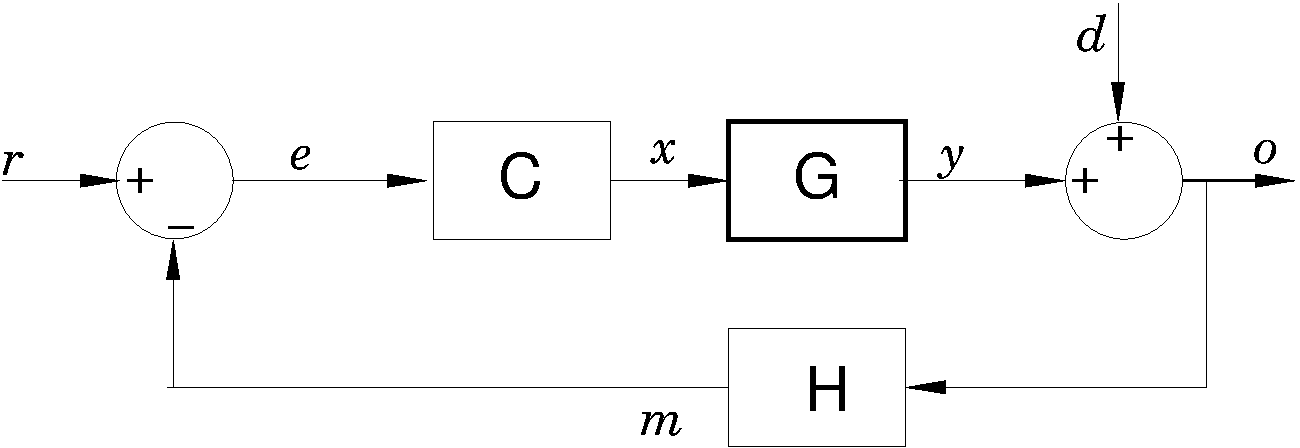
\includegraphics[scale=0.7]{feedback-loop-3.pdf}
	\caption{Diagrama de blocos de um sistema de controle}
	\label{fig:feedback-nobile}	
	\fdireta{Nobile2013}
\end{figure}

\citeonline{Nobile2013} foi ao encontro de soluções adaptativas para gerenciamento de recursos e na alta disponibilidade de aplicações na computação em nuvem. O trabalho optou por aplicar técnicas de adaptação ainda pouco exploradas nas Computação, mas de reconhecimento há décadas por outras áreas da ciência e engenharia. A técnica utilizada foi a teoria de controle, que conta como uma rica coleção de ferramentas de linguagem matemática. Ferramental que auxilia na descrição do comportamento de sistemas dinâmicos em termos de como eles respondem a diferentes estímulos em regime estacionário e transiente.

Uma das definições de um sistema dinâmico foi feita por \citeonline{tsonis1989}, que definiu como:
\begin{citacao}
	Em termos simples, é um sistema cuja evolução a partir de um estado inicial pode ser descrito por alguma regra(s). Estas regras são convenientemente expressas como equações matemáticas. A evolução de um tal sistema é melhor descrito pelo chamado espaço de estado.
\end{citacao}

Já a definição de \citeonline{willems2013} diz que o adjetivo dinâmico refere-se aos fenômenos com uma reação retardada. Fenômenos com um efeito colateral, com transientes, oscilações, e, talvez, uma abordagem para o equilíbrio. Em suma, os fenômenos são em questão a evolução no tempo. Vemos um sistema dinâmico no contexto lógico de definição simples como um modelo matemático, mas um modelo matemático em que os objetos de interesse são funções do tempo: o universo é um espaço de funções.

Sistemas dinâmicos são usados para modelar fenômenos físicos cujo estado ou descrição instantânea muda com o tempo. Este modelo é utilizado, como por exemplo, na previsão econômica e financeira, modelagem ambiental, diagnóstico médico, o diagnostico equipamento industrial, e uma série de outras aplicações \cite{Dean1991}.

Para \citeonline{Scheinerman1995} a dificuldade é que qualquer coisa que evolui ao longo do tempo pode ser considerado um sistema dinâmico. Em seu livro, \citeonline{Scheinerman1995}, inicia descrevendo sistemas dinâmicos matemáticos, mas para o autor um sistema dinâmico tem duas partes: um vetor de estado que descreve exatamente o estado de algum sistema real ou hipotético, e uma função (ou seja, uma regra) que nos diz, dado o estado atual, o que o estado do sistema será no próximo instante de tempo.

É possível representar sistemas físicos (eletrônicos, químicos e biológicos), mas para fins didáticos e em geral, é comum utilizar de sistemas mecânicos e eventos rotineiros para exemplificar a dinâmica dos sistemas:

\begin{description}
	\item[Uma chaleira em aquecimento:] Imagine uma chaleira com água em um fogão convencional em contato a uma chama (tudo sob condições normais de temperatura e pressão), a água presente dentro da chaleira não saltará imediatamente para a temperatura final da chama, pelo contrário, a água do recipiente mostra um aquecimento gradual. O mesmo ocorrerá, mas de maneira inversa, quando a chama do fogo for apagada, a temperatura da água não sofrerá uma queda brusca imediatamente mas, lentamente diminuirá até a temperatura ambiente.
	
	\begin{figure}[htb]
		\centering
		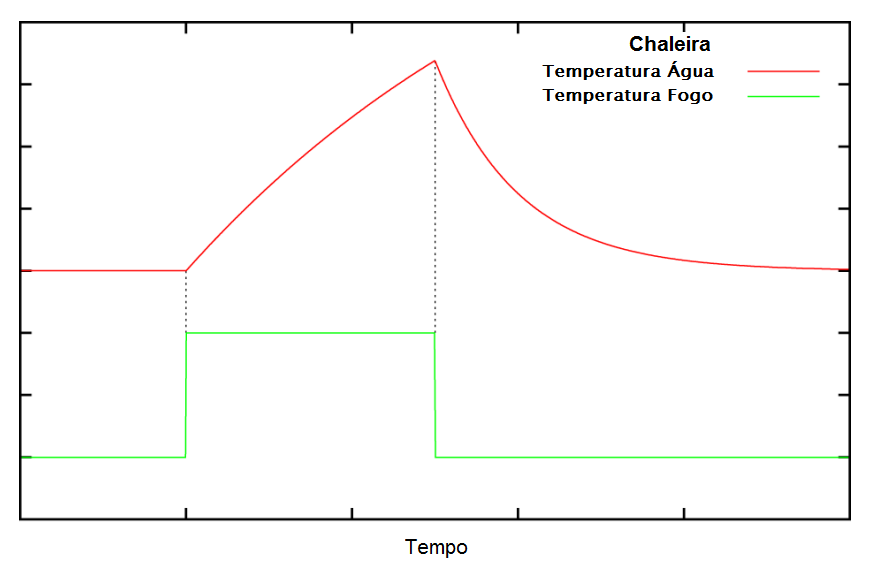
\includegraphics[scale=0.5]{grafico-chaleira.png}
		\caption{Dinâmica e comportamento da chaleira aquecendo}
		\label{fig:chaleira}
		\fdireta{Janert2013}
	\end{figure}
	
	Neste caso da chaleira em aquecimento, o aumento e a constante temperatura da chama (enquanto o fogo ligado, fornecendo calor) representa a entrada do sistema, como indicado pela linha verde da Figura \ref{fig:chaleira}, e o aquecimento da água representa o comportamento do sistema mediante a entrada, conforme demonstrado pela linha vermelha da Figura \ref{fig:chaleira}. 
	
	\item[Uma massa em uma mola:] Agora considere uma massa, em repouso, suspensa por uma mola, também em repouso e fixa em uma superfície plana. Ao deslocarmos o peso tirando-o do repouso e soltarmos após o tencionamento da mola, a massa iniciará uma oscilação até o instante em que a massa e a mola voltarem ao equilíbrio inicial.	
	
	\begin{figure}[!htb]
		\centering
		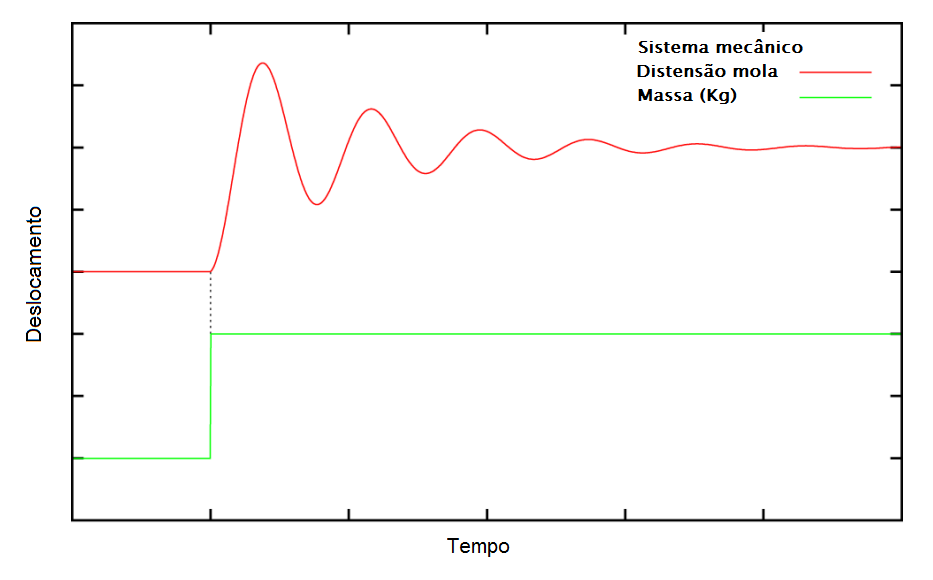
\includegraphics[scale=0.5]{grafico-mola.png}
		\caption{Dinâmica e comportamento da mola}
		\label{fig:mola}		
		\fdireta{Janert2013}
	\end{figure}
	
	O deslocamento inicial (entrada do sistema), por nós provocados, é representado pela linha verde na Figura \ref{fig:mola} e a oscilação subsequente em resposta à força aplicada é representado pela linha vermelha no mesma Figura \ref{fig:mola}.
\end{description}

Os exemplos de sistemas dinâmicos, apresentados anteriormente, e as suas respostas aos estímulos externos, são comportamento comuns em sistemas computacionais e estes aspectos são negligenciados em muitos sistemas, pois até então os sistemas computacionais tem-se comportado com uma dinâmica imperceptível aos usuários. Entretanto, os atuais sistemas computacionais tem tomado tamanha proporção que já não tem respondido imediatamente a uma oscilação na carga de trabalho, apresentando características de dinâmica \cite{Janert2013}, como demonstrado pelo trabalho de \citeonline{Nobile2013}, que apresenta as características dinâmicas de um ambiente de computação em nuvem de larga escala e com impacto apreciável no desempenho dos mecanismos de provisão de QoS.


Embora a análise transiente ainda seja pouco explorada frente as principais abordagens de avaliação de desempenho, \citeonline{Lourenco2015} discute sobre o tema e sua importância para sistemas computacionais. A abordagem predominante à avaliação de desempenho dos sistemas computacionais considera na análise da capacidade no estado estacionário. Geralmente se deseja descartar efeitos de inicialização e, em seguida medir o desempenho quando a saída se estabilizou. A razão para a proeminência na análise estacionária é devido a não importância da dinâmica em sistemas computacionais tradicionais. Normalmente, as plataformas de computação respondem suficientemente rápido as alterações operacionais que afetem o desempenho. Estas justificativas, no entanto, não são necessariamente verdade para sistemas distribuídos emergentes, especialmente em ambientes de grande escala e aplicações de vários níveis. O efeito de pequenos atrasos e a propagação para outras camadas podem render comportamento dinâmico significativos \cite{Lourenco2015}.

Durante o regime transitório, o desempenho pode apresentar comportamentos diferentes, dependendo da dinâmica do sistema: ele pode variar abruptamente, ou lenta e progressivamente, e até mesmo presentes componentes oscilatórios. Análise em regime transitório pode revelar capacidade dinâmica do sistema dependendo das suas propriedades inerciais \cite{Lourenco2015}.

Segundo \citeonline{Janert2013}, a resposta de um sistema a uma perturbação externa muitas vezes consiste em um componente transiente, que desaparece ao longo do tempo, e um componente de estado estacionário. Como demonstrados anteriormente, os componentes diluem no decorrer do tempo, caracterizando-os como transitórios. 

Este conjunto de exemplos tem por objetivo mostrar a importância da avaliação de desempenho principalmente quando um sistema se encontra no regime transiente, pois podem influenciar diretamente no desempenho do sistema. Na avaliação de desempenho de sistemas computacionais em regime transiente é muito comum a irrelevância e o desprezo quando um sistema apresenta \textit{warm-up} \newword{\textit{warm-up}}{período em que o sistema se encontra em regime transiente} principalmente quando a avaliação se concentra em analisar o regime estacionário do sistema o que nem sempre representa efetivamente o real comportament do sistema. Sendo assim, medidas de interesse de regime transientes, como a amplitude máxima atingida pela resposta do sistema e o tempo de assentamento ou ajuste são interessantes para que se possa medir e analisar o comportamento do sistema \cite{Nobile2013}.

No trabalho de \citeonline{Lourenco2015}, o artigo discute sobre a abordagem de análise de estado estacionário vigente para avaliação de desempenho de sistemas computacionais e apresenta uma abordagem para o planejamento de experimentos de simulação destinados a análise transitória, especialmente em aplicações \textit{multi-tiers}.
Esse trabalho de \citeonline{Lourenco2015} inicia discutindo sobre as propriedades dinâmicas de sistemas computacionais de grande escala em ambientes distribuídos e como estas características podem afetar o desempenho. As dinâmicas emergentes da interligação de sistemas computacionais de \textit{multi-tiers} e escaláveis podem produzir efeitos transitórios sobre o desempenho, como resposta temporal e comportamento oscilatório, sendo que estes efeitos variáveis no tempo podem afetar a capacidade de resposta, eficiência e até mesmo a estabilidade do mesmo. 

\begin{citacao}
	Nesse contexto, técnicas de identificação de sistema, análise dinâmica, refere-se à estrutura matemática utilizada para identificar e representam as propriedades dinâmicas de sistemas que apresentam um comportamento inercial, tais como reação e oscilatório amortecido \cite{Lourenco2015}. 
\end{citacao}

Embora a avaliação de desempenho em sistemas computacionais se estabeleceu como um campo de pesquisa nas últimas décadas, esta não adequa-se para sistemas dinâmicos, em geral à avaliação de desempenho de sistemas computacionais considera análise da capacidade em estado estacionário onde se descarta os efeitos de inicialização e, em seguida mede o desempenho quando a saída já se estabilizou. Em um cenário comum, em que a avaliação necessita responder a perguntas como, \textit{Qual a quantidade de carga de trabalho pode a alcançar do sistema antes de degradar excessivamente ?}, ou, \textit{Qual o é o desempenho do sistema com uma determinada carga de trabalho ?}, para uma estimativa quantitativa este experimento é suficiente para expor o sistema \cite{Lourenco2015}.
Como pode-se entender, a análise estacionária na avaliação de desempenho em sistemas computacionais é devido a não importância da dinâmica no sistema. Normalmente, os sistemas são suficientemente rápidos para responder as alterações que afetam o desempenho. Especialmente em ambientes computacionais de grande escala e aplicações de \textit{multi-tiers}, o efeito de pequenos atrasos e propagação para com muitos subsistemas interligados pode render comportamento dinâmico significativo e apreciável, como efeitos inerciais na resolução de tempo de resposta.

Durante os períodos descartados na avaliação estacionaria, o chamando regime transitório, o desempenho pode apresentar comportamentos diferentes, dependendo da dinâmica do sistema, variando abruptamente, lentamente, ou até mesmo presentes comportamentos oscilatórios. Contrastando a identificação do sistema de estado estacionário, um modelo analítico deste tipo prevê o desempenho em função da carga de trabalho e tempo.

Ainda no mesmo trabalho, \citeonline{Lourenco2015} apresenta um conjunto de requisito que especificam uma arquitetura conceitual, intitulada MEDC (\textit{Monitor, Effector, Demanda and Capacity}) representado pela figura \ref{fig:extension-block}. O diagrama ilustra a arquitetura que tem quatro preocupações essenciais: \textit{Demand}, \textit{Capacity}, \textit{Monitor} and \textit{Effector}.

\begin{description}
	\item[\textit{Demand}:] é uma referência para a capacidade de modulação e deve ser configurada de modo a especificar a forma como a carga de trabalho muda ao longo do tempo,
	\item[\textit{Capacity}:]  é a disposição análoga no que diz respeito aos recursos do sistema,
	\item[\textit{Monitor}:] desempenha o papel de um sensor e aquisição de dados temporais, sendo seu dever de coletar os dados sobre o sistema e torná-lo disponível,
	\item[\textit{Effector}:] representam os mecanismos de atuação através modulação da capacidade, que serve como uma camada de abstração disponível para a modelagem dos componentes operacionais que afetam a dinâmica \textit{Capacity} e \textit{Demand};
\end{description}

\begin{figure}[!htb]
	\centering
	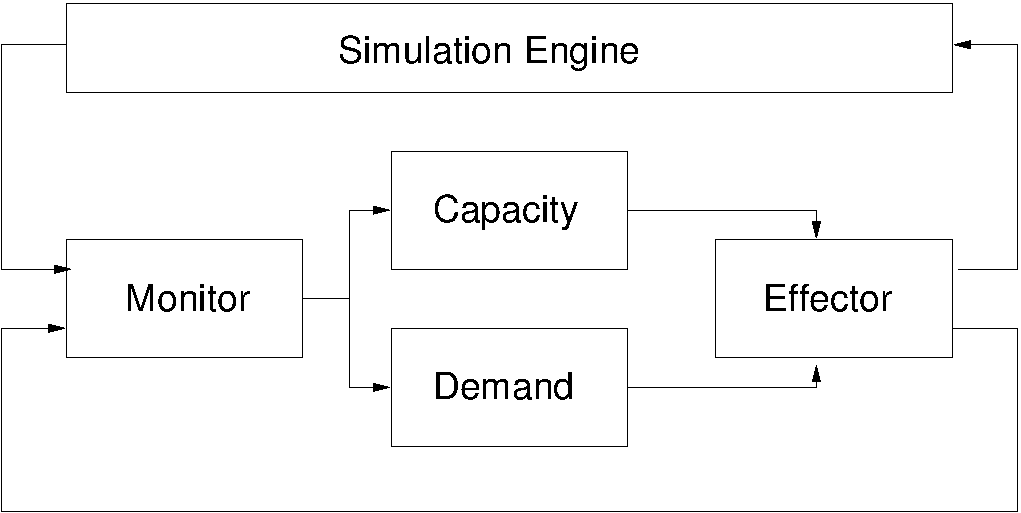
\includegraphics[scale=0.8]{extension-block.pdf}
	\caption{Arquitetura conceitual MEDC}
	\label{fig:extension-block}
	\fdireta{Lourenco2015}
\end{figure}

O fluxo de trabalho, está associado a responsabilidade de controlar a geração de carga com os ciclos de simulação e, correspondentemente, no que diz respeito à capacidade. Este controle se traduz em uma política de tomada de decisão que aciona eventos que solicitam a criação ou o despedimento de novas entidades de carga de trabalho e de recursos. A ordem é efetivamente realizada pelo \textit{Effector}, que recebe as solicitações dos controladores de \textit{Demand} e \textit{Capacity} os manipula antes de transmitir os eventos para o mecanismo de núcleo. É através do \textit{Capacity} que pode-se modelar, por exemplo, atrasos associados a alocação e desalocação, de políticas de escalonamento, enchimento do \textit{buffers}, os tempos de resposta do hardware, padrões de falha de recurso, etc. O dever do \textit{Monitor} está em alimentar a \textit{Demand} e a \textit{Capacity} de dados sobre qualquer estado, por exemplo, utilização média do sistema, tempo de permanência trabalho, relação de perder \textit{deadline}, etc. Para cada uma das quatro responsabilidades, exite uma ação associada de forma iterativa em cada etapa do ciclo de simulação \cite{Lourenco2015}. 

\begin{figure}[!htb]
	\centering
	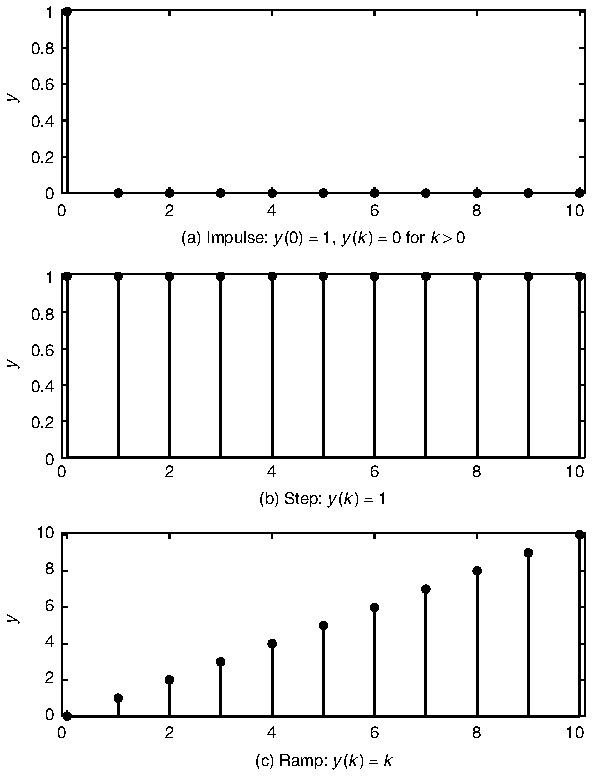
\includegraphics[scale=1.2]{funcoes1.pdf}
	\caption{Sinais em tempo discreto comuns, parte 1}
	\label{fig:funcoes1}
	\fdireta{Hellerstein2004}
\end{figure}

A fim de trazer essas propriedades dinâmicas, a experiência de simulação deve excitar o sistema com carga de trabalho não-estacionária sob condições controladas. Para que seja possível apreciar e apresentar a dinâmica de um sistema e realizar a análise transitória do sistema é preciso utilizar cargas de trabalho que possam provocar comportamentos propícios, onde as caraterísticas dinâmicas do sistema sejam claramente observadas \citeonline{Hellerstein2004}, apresentam propostas de algumas funções, ou sinais, de perturbação, por exemplo: impulso, degrau, rampa, seno, exponencial, seno modulada por uma exponencial, etc.  Essas funções são apresentadas nas figuras \ref{fig:funcoes1} e \ref{fig:funcoes2}.

\begin{figure}[!htb]
	\centering
	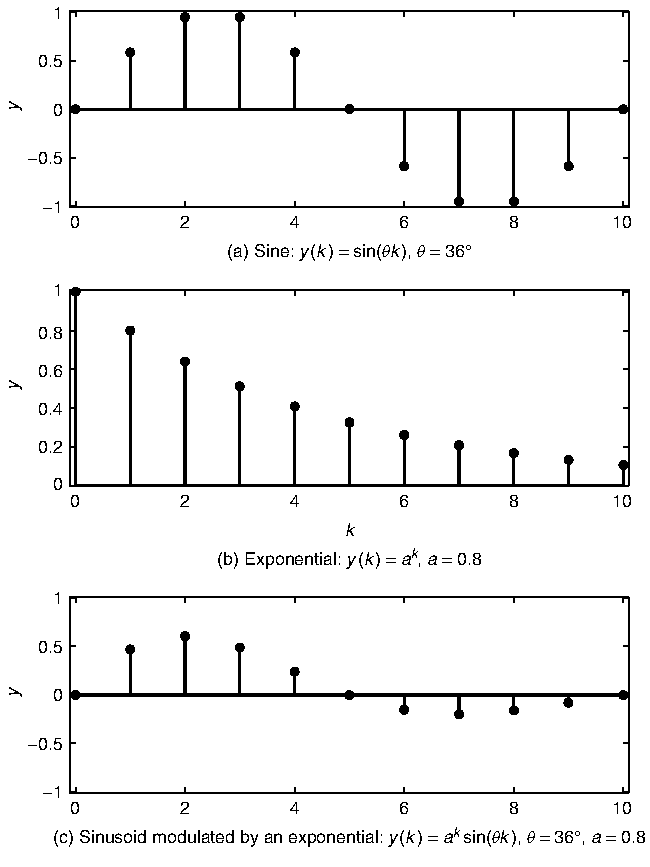
\includegraphics[scale=1.2]{funcoes2.pdf}
	\caption{Sinais em tempo discreto comuns, parte 2}
	\label{fig:funcoes2}
	\fdireta{Hellerstein2004}
\end{figure}

Para a geração de carga para sistemas existem outras propostas que permitem simular um comportamento mais realístico \cite{Mi2010, Mi2009,Mi2008}. Mais especificamente, em \citeonline{Menasce2002}, é apresentada uma outra metodologia para geração de cargas de trabalho que emulam o fenômeno aumento temporal em uma forma controlável. Por exemplo, é de grande interesse fornecer um mecanismo que permite o teste e avaliação do desempenho do sistema sob cargas de trabalho do tipo rajadas. Esta nova metodologia permite injetar quantidades diferentes de rajada dentro do fluxo de chegada utilizando o índice de dispersão. 

Nesse contexto \citeonline{Edwin2015}, pretende utilizar a especificação de arquitetura proposta por \citeonline{Lourenco2015} em um ambiente real. Este trabalho irá atuar diretamente no requisito \textit{Demand} da arquitetura conceitual MEDC, este requisito será implementado em um \textit{benchmark} definido por \citeonline{Edwin2015}.

\textit{Benchmarking} é o principal método para medir o desempenho de uma máquina ou sistema. O \textit{benchmarking} refere-se à execução de um conjunto de programas representativos em diferentes computadores e redes, medindo os resultados. Esses resultados são utilizados para avaliar o desempenho de um determinado sistema com uma carga de trabalho bem definida \cite{Menasce2001}.

O \textit{benchmarking} pode ser visto como um modelo de identificação de oportunidades com o intuito de aumentar a competitividade em ambientes gradativamente turbulentos, assim teve seu surgimento a partir da década de 70 e, tornou-se importante devido às falhas dos métodos tradicionais de fixação de metas que algumas empresas americanas adotavam para enfrentar a concorrência externa, principalmente pelos produtos japoneses \cite{Camila2008}. Para \citeonline{Marco2012} \textit{benchmarks} são um padrão de ferramentas que permitem avaliar e comparar diferentes sistemas ou componentes de acordo com características especificas, tais como desempenho, confiabilidade e segurança. Segundo \citeonline{Folkerts2013} \textit{benchmarks} são ferramentas para responder a uma pergunta \textit{"Qual é o melhor sistema em um determinado domínio?"} ou  \textit{"Qual é o melhor processador?"} ou ainda responde à pergunta \textit{"Qual é o melhor sistema de banco de dados para OLTP?"}. Para \citeonline{Folkerts2013}, a interpretação concreta do \textit{"qual o melhor"} depende do objetivo do \textit{benchmarking}, e esta deve ser a primeira pergunta a ser respondida na concepção de um novo \textit{benchmark}. 


Segundo \citeonline{Stefan2010} a definição de um \textit{benchmarking} é o ato de medir e avaliar o desempenho computacional, sob condições de referência e em relação a uma avaliação de referência. O objetivo do \textit{benchmarking} é permitir a comparação equitativa por diferentes soluções, ou entre desenvolvimentos subsequentes de um sistema em teste SUT. Estas medidas incluem métricas principais de desempenho caracterizando o ambiente em que o SUT está hospedado.

A \textit{Xerox Corporation} é geralmente creditada com o início dos primeiros projetos de avaliação de desempenho global, em 1979. Alertado por uma suspeita de que os custos de produção de máquinas fotocopiadoras foram significativamente mais elevados nos EUA do que no Japão, estas iniciativas \textit{benchmarking} foram utilizados pela Xerox para obter direitos quanto aos materiais, processos e métodos utilizados pelos japoneses. Uma aplicação das lições aprendidas através de \textit{benchmarking} permitiu a \textit{Xerox} aumentar a eficiência de design e produção, e, consequentemente, para reduzir os custos de fabricação de suas máquinas fotocopiadoras. Isto não só reforça a posição de competitiva da \textit{Xerox} no mercado, mas também levou ao desenvolvimento e evolução de uma nova ferramenta gerencial, conhecida como processo de \textit{benchmarking} \cite{Mahmoud2002}.

No contexto de sistemas de simulação, \textit{benchmark} é um software capaz de gerar carga de trabalho a ser aplicada a um sistema computacional com o objetivo de gerar dados acerca de uma métrica de forma que seja possível medir e comparar o desempenho de sistemas sob observação. Para os fabricantes de novos produtos, um \textit{benchmark} pode fornecer informações estatísticas importantes para que eles possam ser ajustados antes da sua implantação. Por outro lado, para os usuários finais, permite ter um ponto de referência na comparação entre pontos fortes e fracos de diferentes produtos. \textit{Benchmarks} ajudam em estimativas de escalabilidade em termos do número de usuários e/ou operações que um sistema pode suportar, e os tempos de resposta do sistema sob várias cargas e plataformas de implantação em hardware/software \cite{Jutla1999}.

O desenvolvimento de um bom \textit{benchmark} tem sido considerada uma "arte negra" por um longo tempo, devido as inumaras sutilezas que influenciam o sucesso do \textit{benchmark}. 
No entanto, pesquisas e estudos com base em \textit{benchmarks} para sistemas computacionais não são um tema novo, para explorar o caminho que levará à uma boa metodologia de extensão, começamos por rever as propriedades pertinentes de um \textit{benchmark}, assim a metodologia incorporará dessas boas práticas para o objetivo de extensão.
As definições de um \textit{benchmark} são temas para uma série de trabalhos que tentam fornecer orientações sobre o assunto, as investigações relacionadas sugerem uma série de orientações amplamente aceitas e critérios de qualidade que devem ser considerados no projeto e execução de \textit{benchmark}, como os trabalhos publicados por \citeonline{Kistowski2015}, \citeonline{Chen2014}, \citeonline{Folkerts2013}, \citeonline{Marco2012}, \citeonline{Huppler2009} e \citeonline{Gray1992} que tem identificado as seguintes características:


\begin{description}
	\item[Relevância] é, talvez, a característica mais importante de um \textit{benchmark}. Mesmo que a carga de trabalho seja perfeita em todos os outros aspectos, será de uso mínimo se ele não fornecer informações relevantes para seus usuários. No entanto, a relevância é também uma característica de como os resultados do \textit{benchmark} são aplicados; \textit{benchmarks} podem ser altamente relevantes para alguns cenários e ter mínima relevância para outros, para o usuário do \textit{benchmark}, uma avaliação da relevância de um ponto de referência deve ser feita no contexto da utilização prevista desses resultados para o \textit{benchmark} \cite{Kistowski2015}. 
	
	\item[Reprodutibilidade] a capacidade de produzir os mesmos resultados de forma consistente para um ambiente de teste em particular, inclui a consistência e capacidade para um outro testador reproduzir de forma independente os resultados em outro sistema. A capacidade de reproduzir os resultados em outro ambiente de teste é em grande parte ligada à capacidade de construir um ambiente equivalente. \textit{Benchmarks} de indústria requerem além de resultados uma descrição do ambiente de teste, geralmente incluindo hardware e componentes de software, bem como opções de configuração, da mesma forma que a pesquisa publicada, que inclui resultados de \textit{benchmark} geralmente inclui uma descrição do ambiente de teste que produziu esses resultados. No entanto, em ambos os casos, a descrição não pode fornecer detalhes suficientes para um laboratório independente ser capaz de montar um ambiente equivalente. \textit{Hardware} deve ser descrito o suficiente em detalhe para uma outra pessoa possa obter um idêntico. As versões de \textit{software} devem ser indicados de modo que seja possível usar as mesmas versões ao reproduzir o resultado. Opções de ajuste e configuração devem ser documentadas para versão do \textit{firmware}, sistema operacional e aplicativo de \textit{software} para que as mesmas opções possam ser usadas quando reexecutar o teste. \cite{Kistowski2015}
	
	\item[Verificabilidade] Dentro da indústria, \textit{benchmarks} são normalmente executados por fornecedores que têm interesse nos resultados. Na academia, os resultados são submetidos a revisão por pares e resultados interessantes serão repetidos e desenvolvidos por outros pesquisadores. Em ambos os casos, é importante que os resultados do \textit{benchmark} sejam verificáveis, de modo que os resultados podem ser considerados dignos de confiança \cite{Kistowski2015}. 
	
	\item[Usabilidade] A maioria dos usuários de \textit{benchmarks} são normalmente técnicos, tornando a facilidade de uso uma preocupação menor do que é para aplicações pensadas e desenvolvidas para o consumidor. Existem, no entanto, várias razões por que a facilidade de utilização seja importante.
	Isso já foi discutido em termos de fazer \textit{benchmark} verificável. Outro aspecto da facilidade de utilização é ser capaz de construir configurações práticas para a execução do \textit{benchmark}. Descrições precisas sobre o hardware do sistema, software e configuração são críticas para a reprodutibilidade, mas pode ser um desafio, devido à complexidade dessas descrições.
	\textit{Benchmarks} podem melhorar a facilidade de utilização, fornecendo ferramentas para ajudar com este processo \cite{Kistowski2015}. 
	
	\item[Escalável] deve ser apoiada em uma maneira que preserve a relação com o cenário de negócios próximo ao modelo real. Além disso, ao usuário deve ser oferecido a possibilidade de dimensionar a carga de trabalho de forma arbitrária pela definição de um conjunto próprio de pontos de escala \cite{Marco2012}. 
	
	\item[Simplicidade] Os elementos conceituais de um \textit{benchmark} devem ser reduzidos ao mínimo e feitos fácil compreensão. O \textit{benchmark} também deve abstrair detalhes que representam configurações de caso a caso, ou escolhas de administração do sistema que não afetam o desempenho \cite{Chen2014}. Um \textit{benchmark} com uma estrutura altamente complexa é muitas vezes difícil de entender e difícil confiar. Se as pessoas não confiam no \textit{benchmark}, elas não vão usá-lo. \textit{Benchmarks} devem, portanto, ser o mais simples possíveis. Complexidade necessária pode ser explicado em uma documentação do \textit{benchmark} \cite{Weber2014}.
	
	\item[Econômico] Ele é muitas vezes negligenciado durante o desenvolvimento inicial do \textit{benchmark}, pois as fases iniciais do desenvolvimento estão focadas em imitar a realidade para fornecer a relevância necessária para o \textit{benchmark}. Na verdade, para ser relevante, pode-se esperar um \textit{benchmark} realístico; e ser realístico, muitas vezes significa ser complexo; e complexo pode ser invariavelmente caro. Esta é claramente uma outra oportunidade para o compromisso, se alguém quiser criar uma \textit{benchmark} de sucesso. O termo "econômico", não significa \textit{"barato"}, mas sim \textit{"vale o investimento"}.
	Considere os resultados da IBM, \sigla{TPC-C}{\textit{On-line Transaction Processing}} ou  \sigla{TPC-E}{\textit{Complex on-line transaction processing}} ou  \sigla{TPC-H}{\textit{Ad-hoc decision support system}} e alguns da \sigla{SPEC}{\textit{Standard Performance Evaluation Corporation}}, SPECjAppServer2004 e  SPECweb2005, todos eles selecionam apenas uma fatia da \textit{"realidade total"} da indústria da informática, no retorno para o apelo de ser barato para correr, fácil de executar e fácil de verificar. Enquanto eles não são usados fora do contexto da sua intenção, eles também atendem aos requisitos para a relevância, equidade e repetibilidade \cite{Huppler2009}. 
	
	\item[Métrica] uma métrica ser claramente compreensível e é obrigada a relatar sobre as reações do SUT referentes à carga. Segundo \citeonline{Folkerts2013} as métricas do \textit{benchmark} devem permitir caracterizar e quantificar o comportamento do sistema quando enfrenta perturbações (ou seja, falhas, ataques, e variações de ambiente operacional). À primeira vista, resiliência métricas de \textit{benchmark} devem caracterizar o desempenho, confiabilidade e segurança \cite{Marco2012}.
	
\end{description}

Nas abordagens mencionadas acima, referentes ás propriedades de um \textit{benchmarks} de sucesso, segundo os autores, nenhum dos trabalhos contemplam uma metodologia de extensão em que o \textit{benchmark} pode ser desenvolvido. Na seção a seguir, este trabalho propõe tal metodologia, e nos capítulos seguintes foi ilustrado através de um estudo de caso a extensão de um \textit{benchmark} usando tal metodologia. É importante compreender as características de uma carga de trabalho e determinar se é ou não aplicável para uma situação particular. Ao desenvolver uma nova carga de trabalho, as metas devem ser definidas para que escolhas entre os critérios de projeto concorrente possam ser feita de acordo com esses objetivos para alcançar o equilíbrio desejado \cite{Kistowski2015}.

Antes de definir a metodologia propriamente dita, é importante assegurar que não é qualquer \textit{benchmark} que pode ser modificado pela extensão, existem alguns pré-requisitos e estes são apresentados. O trabalho de \citeonline{Folkerts2013} apresenta a definição de três grupos de requisitos, com base nas propriedades apresentadas anteriormente:

\begin{description}
	\item[1. Requisitos gerais] - este grupo contém requisitos genéricos. 
	\begin{itemize}
		\item Relevância
		\item Econômico
		\item Simplicidade
	\end{itemize}
	
	\item[2. Requisitos de Implementação] - este grupo contém as exigências relativas à implementação e desafios técnicos. \hfill 
	\begin{itemize}
		\item Fair e portáteis
		\item Reprodutibilidade
		\item Realista
		\item Relevância
	\end{itemize}
	
	\item[3. Requisitos de Carga de Trabalho ] - contém os requisitos quanto à definição de carga de trabalho e suas interações. \hfill 
	\begin{itemize}
		\item Representatividade
		\item Escalável
		\item Métricas
	\end{itemize}
	
\end{description}


O \textit{benchmarking} utilizado neste trabalho e objeto alvo da extensão é o Bench4Q, que simula um \textit{e-commerce} orientado a QoS e oferece recursos para deduzir uma representação controlável e flexível de cargas de trabalho baseadas em sessão complexas, e para simular o comportamento do cliente autêntico \cite{Bench4Q}.

\textit{E-commerce}, que é uma loja virtual de comercio eletrônico, tem se tornado cada vez mais popular e ganhado cada vez mais concorrência com o desenvolvimento e expansão da Internet.O Bench4Q é um \textit{benchmarking} que segue a metodologia de \textit{e-commerce} orientado a QoS, providos de recursos que permitem a simulação de um ambiente controlável e flexível. Além disso, o Bench4Q pode ser usado para avaliar o desempenho de escalabilidade do sistema.

O trabalho \citeonline{cherkasova1998}, apresenta o conceito de sessão, que define uma sequencia de requisições de um único cliente. \citeonline{Krishnamurthy2006}, apresentam a dependência de sessões em sistemas \textit{e-commerce} e ressalta a importância de caracterizar a carga de trabalho sintética.

Apesar do grande sucesso do \sigla{TPC-W}{\textit{Transaction Processing Performance Council - Web}} \footnote{TPC-W: \url{http://www.tpc.org/tpcw/}}, existem diversos trabalhos que apresentam métricas baseadas em sessões mais úteis das quais utilizadas pelo \textit{benchmark}. Ainda assim existe outro conjunto de trabalhos concentrado em como fazer TPC-W ser mais realístico. Em geral, essa obras tem inserido \textit{burstiness} na simulação de carga. O trabalho \citeonline{Mi2009}, incluiu o comportamento de \textit{burstiness}. Enquanto a obra de \citeonline{Sobel2008}, busca adaptar o TPC-W para o ambiente em nuvem.

Embora a grande diversidade dos trabalhos apresentados, o Bench4Q oferece uma solução integrada para \textit{e-commerce} sensíveis a QoS. Vale salientar que, não há nenhuma solução integrado as características, especialmente, a de encontrar qualquer extensão TPC-W sensível a QoS para \textit{e-commerce}. Contudo, existem trabalhos que abordam a modelagem de rajadas no processo de chegada da carga de trabalho imposta ao sistema \textit{e-commerce}. \citeonline{Casale2012}, apresenta o \sigla{BURN}{\textit{BURtiness eNabling method}}, uma metodologia para gerar rajadas customizáveis como demanda de carga de trabalho afim de avaliar o desempenho de um sistemas \textit{e-commerce}. A metodologia BURN é composta de duas políticas tradicional (que gera a carga de trabalho constante, a mesma gerada pelo TPC-W) e a \textit{burst} (que insere as rajadas na carga de trabalho tradicional). Durante a execução do \textit{benchmark}, BURN aplica um stress na aplicação \textit{e-commerce} alternando as duas políticas. Tais trabalhos buscam avaliar o desempenho sistemas de multi-camadas (composto por um servidor de aplicação, base de dados, etc) que hospedem um \textit{e-commerce} como é o caso do Bench4Q.


Sistemas de \textit{e-commerce} tem uma grande preocupação com os níveis de QoS, pois estão relacionados diretamente com os lucros do website. Atualmente a maioria dos \textit{e-commerce} são desenvolvidos sensíveis a QoS. O \textit{e-commerce} do Bench4Q é sensível a QoS.  Com o desenvolvimento da tecnologia Web, o TPC-W se tornou uma referência de \textit{e-commerce}, entretanto a implementação do TPC-W é insuficiente para \textit{e-commerce} sensíveis a QoS.

A maioria dos \textit{benchamarks} de \textit{e-commerce}, incluindo o TPC-W, são limitados para os sistemas sensíveis a QoS. As métricas utilizadas são baseadas em requisições \sigla{HTTP}{\textit{Hypertext Transfer Protocol}}, como a taxa de requisições atendidas com sucesso ou o tempo de resposta das requisições. Embora uma das características mais críticas de um sistema de \textit{e-commerce} sensíveis a QoS seja a integridade do serviço prestado aos clientes, as métricas baseada em requisições podem levar a afirmações ineficientes e até mesmo erradas.

O Bench4q é uma extensão do TPC-W \cite{Menasce2002}, e tem como objetivo o \textit{tuning} de servidores \textit{e-commerce} orientados a fornecer QoS aos seus clientes. As principais características do Bench4Q incluem: 
apoio à análise de métricas baseada em sessão que simula carga sensível a QoS para uma análise da capacidade. 

O \textit{benchmark} Bench4Q, é distribuído de acordo com a \sigla{GNU}{\textit{Lesser General Public License}}, sendo um software livre, ele pode ser redistribuído e/ou modificado sob os termos da licença publicas pela \textit{Free Software Foundation}. Seguindo muitas diretrizes da especificação do TPC-W, o Bench4Q usa principalmente em suas métricas de simulação a garantia de QoS \cite{Bench4Q}. 

O Bench4Q oferece uma arquitetura distribuída para a geração de carga através de seus agentes que são conectados a um único console que os gerencia, entretanto é possível configurar separadamente as configurações para cada agente. Esses agentes geram carga (requisições HTTP) para o servidor de aplicação onde esta hospedado o \textit{e-commerce} como ilustrado na figura \ref{fig:arquitetura-bench4q}. Os resultados da avaliação de carga aplicada ao \textit{e-commerce} são coletados pelo console que apresenta alguns gráficos, que facilitam a interpretação da avaliação mediante as diretrizes do TPC-W que são complexas \cite{Bench4Q}.

A ferramenta é composta por três partes: Console, Agente e SUT, conforme apresenta a figura \ref{fig:arquitetura-bench4q}, e também disponibiliza interfaces para o monitoramento de recursos para o servidor de aplicação e para o banco de dados, este monitoramento inclue CPU, memória, rede, etc.


\begin{figure}[htb]
	\centering
	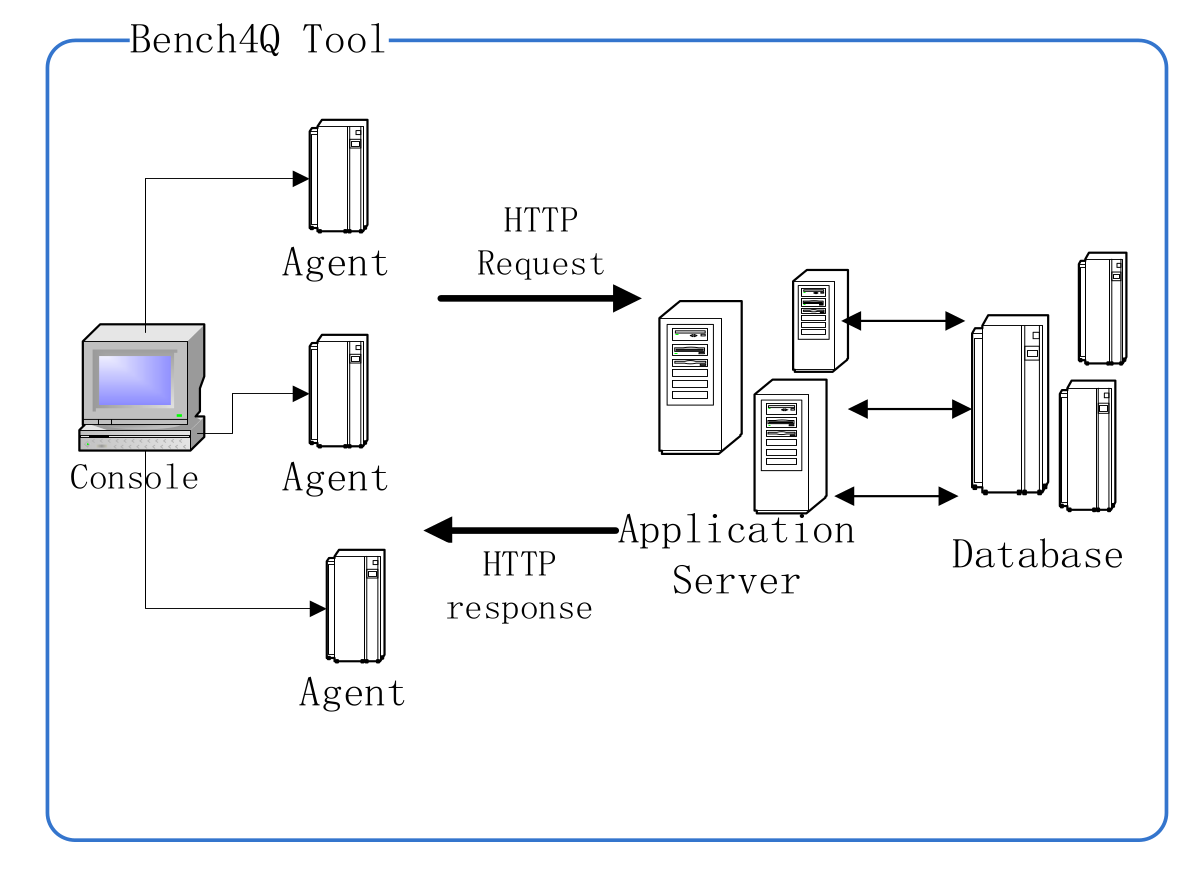
\includegraphics[scale=0.3]{bench4Q.png}
	\caption{Arquitetura Bench4Q}
	\label{fig:arquitetura-bench4q}
	\fdireta{Bench4Q}
\end{figure}

\begin{itemize}
	
	\item \textbf{Console:} A Figura \ref{fig:console-bench4q} apresenta a interface do console, onde configura-se o teste, coleta e exibe os resultados. 
	
	\begin{figure}[!htb]
		\centering
		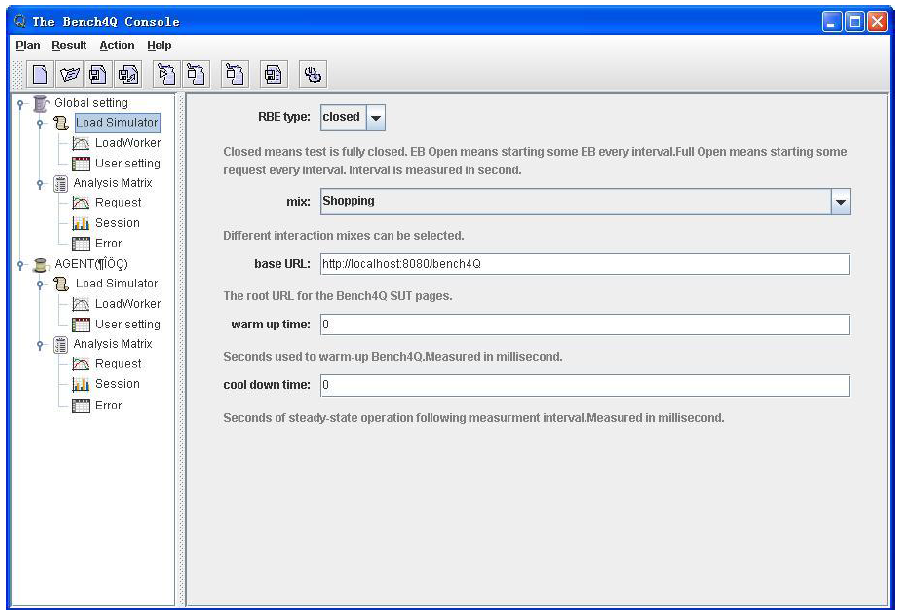
\includegraphics[scale=0.7]{console-bench4Q.png}
		\caption{Console Bench4Q}
		\label{fig:console-bench4q}
		\fdireta{Bench4Q}	
	\end{figure}
	
	\item \textbf{Agente:} É este que faz o trabalho real, pois gera a carga configurada no console. Simula o comportamento dos usuários no \textit{website}, disparando diversas requisições para o \textit{e-commerce}. 
	
	\item \textbf{SUT:} O \textit{e-commerce} SUT (\textit{System Under Test}), conforme apresentado na figura \ref{fig:sut},  é quem fornece o website de compras e está organizado com um banco de dados, servidor web e servidor de aplicativos. O portal compreende todos os componentes que fazem parte de uma aplicação real, isso inclui as conexões de rede, servidores web, servidores de aplicação, servidores de banco de dados, etc.
	
	\begin{figure}[htb]
		\centering
		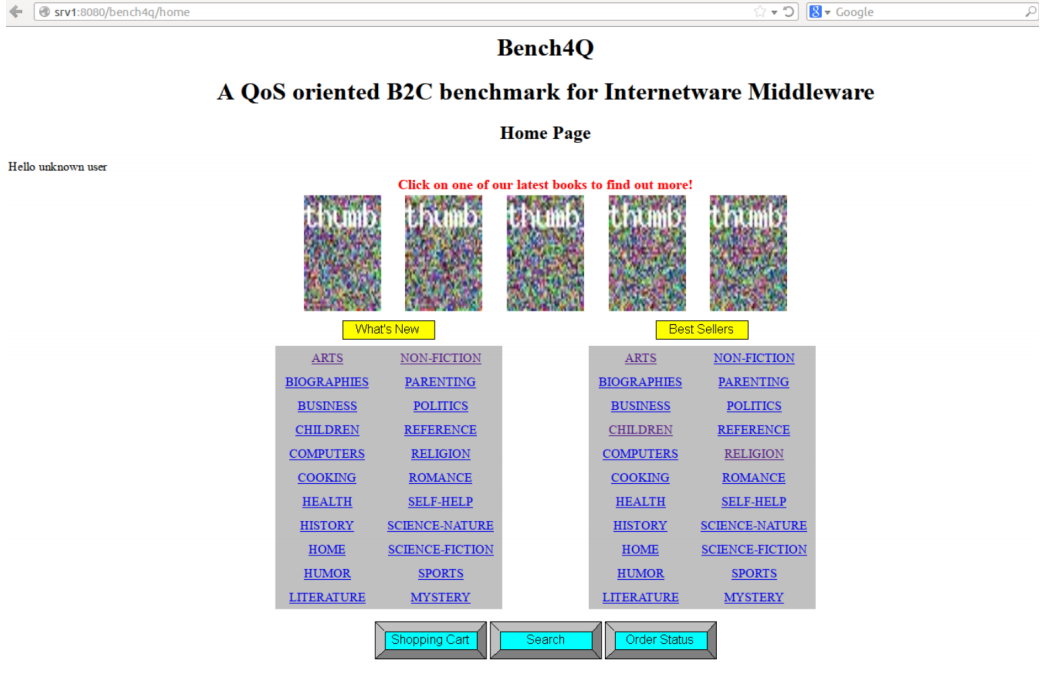
\includegraphics[scale=0.51]{sut.png}
		\caption{SUT Bench4Q}
		\label{fig:sut}
		\fdireta{Bench4Q}
	\end{figure}
	
\end{itemize}

De uma maneira mais especifica, percebe-se que os \textit{benchmarks} para aplicações computacionais típicas de computação em nuvem, como \textit{e-commerce}, por exemplo, não são atualmente orientados a suportar totalmente QoS %, porque alguns recursos de QoS críticos não podem avaliados por eles
\cite{Zhang2011}. Um exemplo desses recursos é a integralidade do serviço, que é geralmente expressa como uma sessão fornecida aos clientes. Nesse sentido o Bench4Q tenta abranger essa lacuna.


O TPC-W, estendido pelo Bench4Q, é (mesmo atualmente tido como obsoleto) um \textit{ benchmark} direcionado a \textit{sites} de \textit{e-commerce} transacionais em que os consumidores são vinculados a sessões, cada cliente possui sua própria e única sessão em determinado intervalo de tempo. Trata-se de um site de venda de livros implementado em Java e hospedado em um servidor de aplicação Tomcat \footnote{Tomcat: \url{http://tomcat.apache.org/}}. Clientes, intitulados pela ferramenta como \textit{browsers}, são emulados e se comportam como consumidores dos produtos oferecidos pela loja virtual. Basicamente, os clientes podem interagir de diferentes formas: acessar a página inicial do \textit{site} (home), navegar e procurar por produtos, realizar operações que envolvam o carrinho de compras e finalizar uma compra. A carga de trabalho gerada pelo TPC-W pode ser representada por um \sigla{CBMG}{\textit{Customer Behavior Model Graph}}, um grafo orientado, em que os nós representam uma operação a ser realizada (procurar, navegar, comprar etc.) e os pesos nas arestas significam a probabilidade de transição de uma operação para outra \cite{Zhang2011}. A Figura \ref{fig:CBMG} modela o fluxo de requisições a páginas e operações que um cliente pode realizar em uma sessão, basicamente um comportamento estocástico de acesso às páginas.

\begin{figure}[htb]
	\centering
	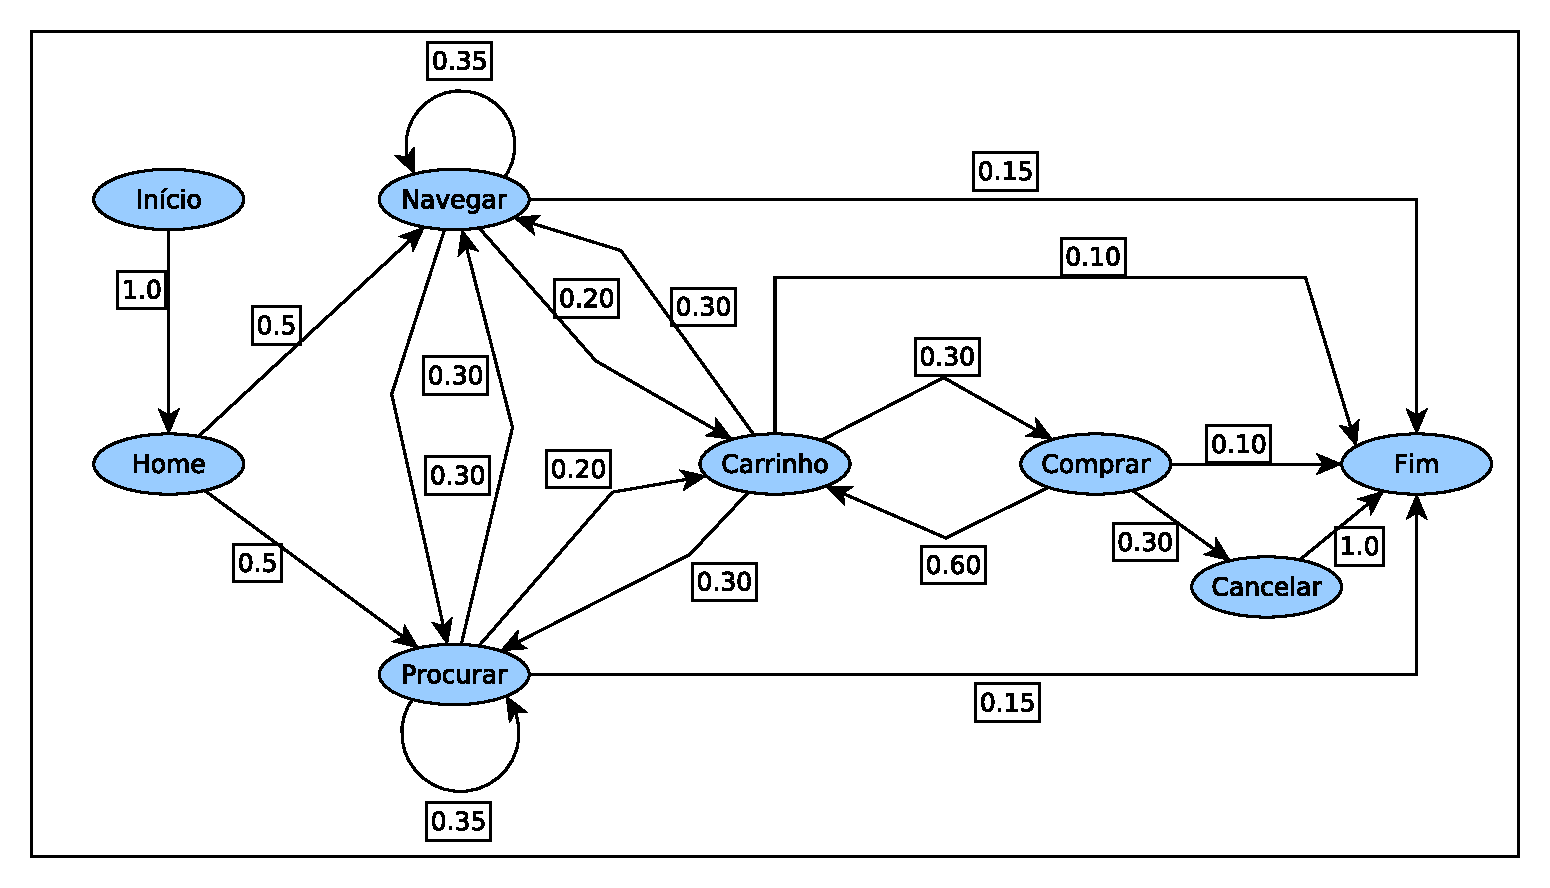
\includegraphics[scale=0.6]{CBMG.pdf}
	\caption{CBMG - perfil de navegação dos \textit{brwosers} do Bench4Q}
	\label{fig:CBMG}
	\fadaptada{Mark2007}
\end{figure}


A carga de trabalho gerada pelo TPC-W é formada por um CBMG com 14 tipos de interação \textit{web} e três perfis de pesos para suas arestas. O resultado é uma carga em que a maioria dos clientes apenas navega nas páginas (navegação: $95\%$ e compra: $5\%$); outra em que a maioria dos clientes realiza compras de forma moderada (navegação: $80\%$ e compra: $20\%$); e a terceira composta por muitos clientes que finalizam as compras (navegação: $50\%$ e compra: $50\%$). Vale ressaltar que existe um atraso entre as requisições de uma sessão. Ao iniciar uma sessão uma requisição é disparada e após receber a respectiva resposta, a próxima requisição acontece após um tempo também estocásticos e variante. Essa especificação tem o objetivo de emular melhor o comportamento humano ao acessar \textit{sites} de \textit{ e-commerce}.

Ao ser implantado em uma infraestrutura computacional que hospede todos seus componentes, os clientes emulados devem estar localizados fora de tal infraestrutura e conectados por uma rede. Estes clientes começam as séries de requisições. O TPC-W implementa um modo de geração de carga conhecido como fechado (\textit{close mode}): um novo cliente chega somente após o antigo deixar o sistema \cite{Zhang2011}. As métricas disponíveis concernem basicamente sobre a quantidade de interações \textit{web}, medidas em quantidade por segundo (\sigla{WIPS}{\textit{ Web Interaction Per Second}}) e seu tempo de resposta (\sigla{WIRT}{\textit{Web Interaction Response Time}}).

A motivação para a extenção do TPC-W e criação do Bench4Q começa porque, muito embora, as referidas métricas aparentem descrever bem a quantidade de acessos ao sistema, a qualidade do serviço experimentada pelo usuário pode ser desproporcional a essas mesmas métricas. Em \citeonline{bench4qslides} é descrito um ensaio que contempla dois cenários diferentes: um normal e outro otimizado não realisticamente. A otimização foi feita pela configuração de parâmetros no servidor Tomcat, a saber: \texttt{sessionTimeout}, \texttt{connectionTimeout} e \texttt{acceptCount}. Um das características da aplicação é a presença de operações \textit{ IO-bound}, por consequência, observar o tempo médio de resposta dessas operações permite diminuir os valores de estouro de tempo, e, com isso, forçar uma taxa de utilização de CPU. Assim, pode-se ``otimizar'' o ambiente da aplicação. Os resultados foram de $WIPS = 131$ para o cenário normal e $WIPS=199$ para aquele otimizado não realisticamente, colaborando com a hipótese. Porém, ao observar a quantidade de sessões completadas com sucesso, conforme apresentado na figura \ref{fig:seeing}, percebe-se que o cenário normal permitiu uma quantidade de erros menor do que aquele otimizado não realisticamente. Por consequência, uma espectativa de lucro maior quando da implantação: maior quantidade de sessões realizadas sem error implicaria em maior probabilidade de compras efetivas.

\begin{figure}[htb]
	\centering
	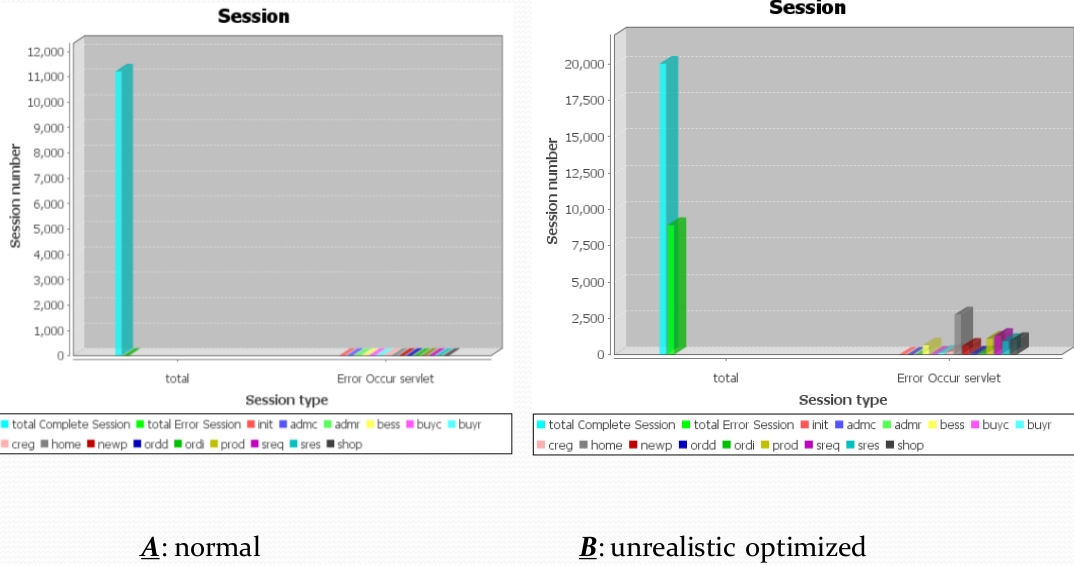
\includegraphics[scale=0.45]{seeing.png}
	\caption{Comparação da quantidade de requisições completadas com sucesso entre dois cenários: normal e otimizado não realisticamente.}
	\label{fig:seeing}
	\fdireta{Bench4Q}
\end{figure}


Tanto o TPC-W quando Bench4Q tem como objetivo produzir resultados que possibilitem o \textit{tuning} (sintonia do parâmetros) de servidores que compõem serviços de \textit{e-commerce} orientados a fornecer QoS aos seus clientes \cite{Menasce2002, Zhang2011}.  A ideia principal é que seja construída uma banca de testes (\textit{testbed}), haja a execução do \textit{benchmark} e consecutiva geração dos traços de execução, seja feita a extração dos dados e, por fim, com base nos resultados, melhores valores para os parâmetros de configuração do sistema sejam aplicados. Especificamente sobre o Bench4Q, as principais funcionalidades implementadas nele tem como contexto a observância do estado das sessões.
%}

%Neste capítulo será apresentado o \textit{benchmark} Bench4q que foi desenvolvido pelo \textit{Technology Center of Software Engineering} da \textit{Chinese Academy of Sciences} no \textit{Institute of Software}.
O \textit{e-commerce} é um modelo de negócio bastante comum e possível principalmente por sua implantação em ambiente \textit{ web}, orientado a negociação de bens e serviços. Igualmente como o que acontece na forma tradicional de negociação, disputas por clientes e/ou fatias de mercado surgem naturalmente, como podem ser observadas em promoções, ofertas, lançamentos de novos produtos etc. Portanto, um \textit{ website} alinhado a esses requisitos que proporcionem um desempenho melhor, ou seja, que possibilidade uma experiência melhor a seus usuários, certamente já possui uma vantagem competitiva. Nesse sentido, o desempenho da infraestrutura que hospedará o negócio e o ajuste fino dos parâmetros operacionais da solução de \textit{e-commerce} podem ser encarados como requisitos não-funcionais. Assim, seria possível realizar avaliações de desempenho que fomentem o projeto de tais sistemas cujo resultado sejam sistemas mais eficientes, mesmo que sejam abstraídas algumas regras específicas do negócio a ser implementado. O Bench4Q é uma ferramenta que possibilita tais projetos.

A oscilação da carga de trabalho é uma característica fundamental. A simultaneidade dos acessos apresentam grandes efeitos sobre a escolha da política de ajuste de um servidor, o Bench4Q simula tal oscilação de carga através dos seus agentes com os seguintes parâmetros:

\begin{itemize}
	\item \textit{Base Load:} Quantia fixa de \textit{threads} por agentes.
	\item \textit{Radom Load:} Quantidade de \textit{threads} que são geradas aleatoriamente.
	\item \textit{Rate:} O \textit{rate} (taxa de mudanças de carga), pode ser positivo, negativo ou nulo. Positivo significa que a carga de base está aumentando a cada segundo, se negativa significa que a carga de base está diminuindo a cada segundo e enquanto a taxa é zero, a carga é fixa.
	\item \textit{Trigger Time:} O tempo para o agente de carga para começar a gerar sua carga.
	\item \textit{Duration:} O tempo de execução do agente de carga.
\end{itemize}

%As composições as cargas simuladas por diversos agentes, podem gerar as seguintes flutuações de carga típicas de empresas B2C podem ser simulados.

\begin{figure}[htb]
	\centering
	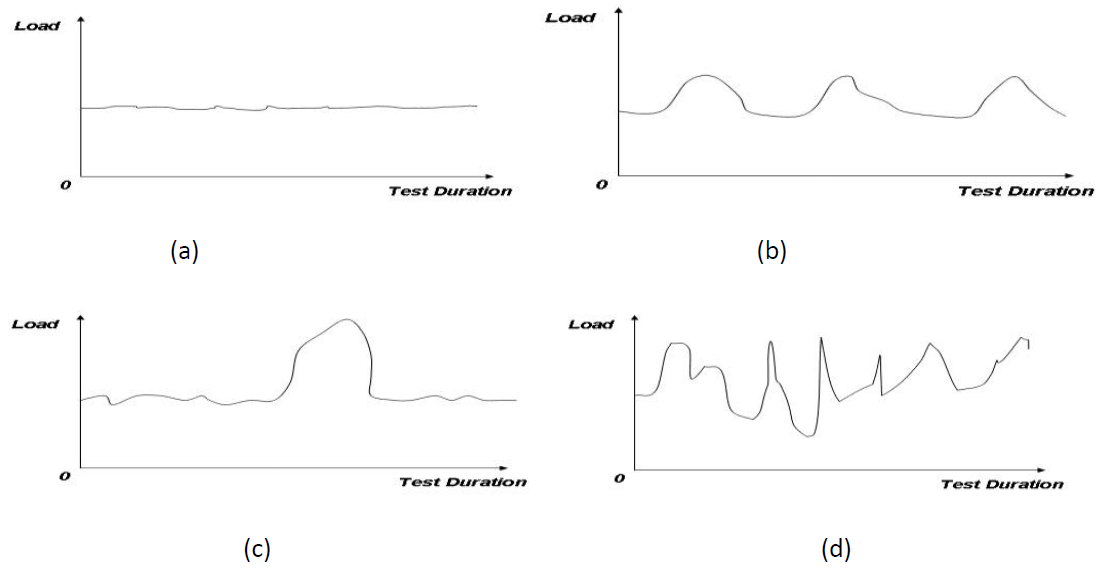
\includegraphics[scale=0.5]{load_fluctuation.png}
	\caption{Carga de trabalho gerada pelo Bench4Q}
	\label{fig:carga-gerada}
	\fdireta{Bench4Q}
\end{figure}


Existe dois modos de simulação de carga, o fechado e o aberto, conforme apresentado na figura \ref{fig:type-session}. No modo fechado, ilustrado na figura \ref{fig:type-session} (a), um novo cliente só acessará depois do cliente antigo deixar o sistema. Já o modo aberto, ilustrado na figura \ref{fig:type-session} (b), novos clientes vão acessar o sistema sem se importar com a saída dos antigos clientes. O TPC- W simula carga no modo fechado, o que faz uma suposição inexistente do mundo real \cite{Bench4Q}. 

\begin{figure}[htb]
	\centering
	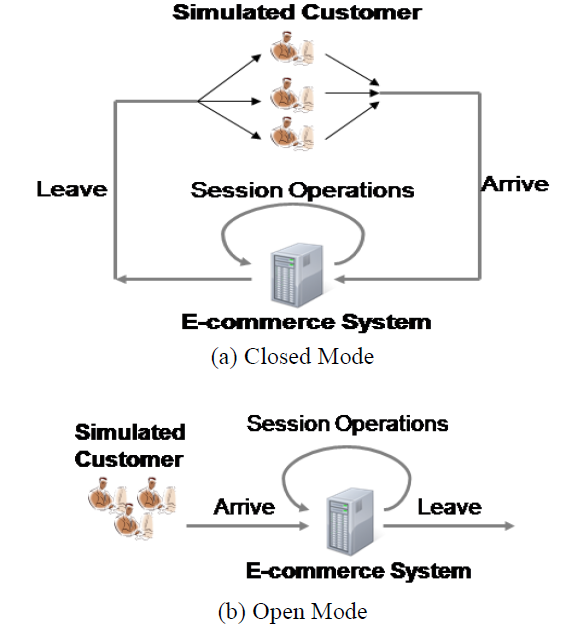
\includegraphics[scale=0.6]{type_session.png}
	\caption{Tipo de sessões Bench4Q}
	\label{fig:type-session}
	\fdireta{Bench4Q}	
\end{figure}


Em sistemas baseados em sessões reais, como a proposta deste projeto, os clientes vêm com base em um modo aberto. Em sua utilização neste projeto, a sessão aberta é a que mais se adéqua a finalidade do objetivo proposto.


%definição para fisicos - Dynamical systems in cosmology
%O que é um sistema dinâmico? Pode ser qualquer coisa que vão desde algo tão simples como um único pêndulo para algo tão complexo como o cérebro humano e todo o próprio universo. Em geral, um sistema dinâmico pode ser considerado como qualquer sistema que consiste em resumo
%1. um espaço (espaço de estados ou espaço de fase), e
%2. uma regra matemática que descreve a evolução de qualquer ponto nesse espaço.
%O segundo ponto é crucial. Encontrar uma regra matemática que, por exemplo, descreve a evolução da informação em qualquer neurônio no cérebro humano é provavelmente impossível. Então, precisamos de uma regra matemática como uma entrada e encontrar um pode ser muito difícil.
%O estado do sistema, estamos interessados ​​em é descrito por um conjunto de quantidades que são considerados importantes sobre o sistema, eo espaço de estado é o conjunto de todos os valores possíveis destas quantidades. No caso do pêndulo, a posição da massa e a sua quantidade de movimento são quantidades naturais para especificar o estado do sistema. Para sistemas mais complicados, como o universo como um todo, a escolha de boas quantidades não é de todo óbvio e ele acaba por ser útil para escolher variáveis ​​convenientes. É possível analisar o mesmo sistema dinâmico com diferentes conjuntos de variáveis, cada um dos quais pode ser mais apropriado a uma questão particular.
%Existem dois tipos principais de sistemas dinâmicos: A primeira são sistemas dinâmicos contínuos cuja evolução é definida por um conjunto de equações diferenciais ordinárias (EDOs) e os outros são chamados de sistemas dinâmicos em tempo-discreto que são definidos por um mapa ou equações de diferença. No contexto da cosmologia estamos estudando as equações de campo de Einstein que para um resultado homogêneo e isotrópico espaço em um sistema de equações diferenciais ordinárias. Assim, estamos interessados ​​apenas em sistemas dinâmicos contínuos e não discutirá sistemas dinâmicos em tempo-discreto no restante


% Nobile
%Em geral, é possível representar sistemas físicos (e. g. eletrônicos, químicos e biológicos) por equações diferenciais obtidas a partir leis básicas da Física. Esses sistemas de equações diferenciais descrevem uma determinada dinâmica do sistema no domínio do tempo e, com o desenvolvimento dessas equações, é possível identificar propriedades fundamentais para o projeto de controle.
%Nas engenharias sistemas mecânicos são bastante semânticos e amplamente utilizados como exemplo na modelagem de sistemas. A figura 3.5 ilustra um sistema mecânico massa-mola simples onde um objeto de massa m está preso a uma mola cuja constante de elasticidade é igual a k fixa em uma superfície plana. Para simplificar a modelagem, considerações podem ser feitas, como supor que o sistema está livre da influência de outras forças.


%\cite{mytkowicz2009} afirma que  computadores modernos são sistemas dinâmicos não-lineares

%_____________Computer systems are dynamical systems
%Os computadores modernos são sistemas dinâmicos não-lineares complexas. Registos microprocessador, o conteúdo da memória, e até mesmo a temperatura de diferentes regiões do chip são variáveis ​​de estado desses sistemas. A lógica programado em um computador, combinados com o software de execução em que o hardware, define a dinâmica do sistema. Sob a influência dessas dinâmicas, o estado do computador se move em uma trajetória através do seu espaço de alta dimensão estado como o progresso ciclos do relógio eo programa é executado. Chamamos isso a dinâmica de um sistema de computador de desempenho para distingui-lo a partir da dinâmica do programa: a sequência de passos que o código a seguir. Embora a dinâmica do programa são geralmente simples e fácil de entender, a dinâmica de um programa rodando em um computador moderno de desempenho pode ser complexo e até mesmo caótico. As implicações disso não são apenas interessante, mas realmente muito importante, tanto do ponto de vista dinâmica e para os efeitos de simulação computacional e design.
%Este pensamento está em contraste gritante com as abordagens tradicionais na literatura sistemas de computadores, onde os computadores são modeladas como processos estocásticos altos-dimensional, 1,2 detalhes temporais estão aglomeradas em indicadores agregados, 3,4 e os problemas de observação e de perturbação que são inerentes em qualquer experiência do mundo real são evitados através da utilização de simuladores, em vez de hardware.5,6 real dos 364 trabalhos sobre a compreensão do desempenho de inovações microprocessador que apareceu entre 2004 e 2007, em três conferências microarquitetura importantes? ASPLOS, ISCA, e micro ?, por exemplo, apenas nove analisaram o comportamento variável no tempo de hardware real. Enquanto arquitetos de computador fazem perceber os efeitos de não-linearidade, falta-lhes um quadro verdadeiramente princípios para lidar com seus efeitos. Como uma solução parcial, o campo tem utilizado abordagens baseadas no conhecimento? Por exemplo, refs. 10/07? e técnicas fundamentadas em pesquisa e operações de investigação? por exemplo, refs. 11-13 ?. Mesmo assim, o resultado de um novo recurso de design rotineiramente surpreende sua creators.14
%A combinação particularmente pernicioso de não-linearidade e medição perturbação só recentemente foi reconhecido como uma questão importante por computador architects.15,16 computadores modernos têm milhões de transistores que interagem de formas complexas e não-lineares, e quase qualquer medição de seu estado pode perturbar o seu comportamento . Como resultado, a dinâmica de sistemas de computadores de desempenho pode olhar random-dando assim origem e credibilidade à idéia de que a evolução do desempenho de um computador acontece a partir de um processo estocástico.
%Como os leitores desta revista estão bem conscientes, no entanto, olhando aleatória e ser aleatório pode ser duas coisas diferentes. A dinâmica de um computador é ditada pelas leis físicas determinísticos de suas partes: fios, semicondutores, e assim por diante. Nem este hardware nem o código que é executado em que é estocástico, e assim parece lógico ter uma abordagem dos sistemas dinâmicos para a análise do seu comportamento acoplado.
%Seguindo este raciocínio, nós tratamos a tarefa de compreender o comportamento de um computador como equivalente a análise da dinâmica de espaço de estado do sistema. Esta abordagem, foi pioneira na Ref. 17, não é apenas uma maneira útil de descrever e compreender estes sistemas; ele também permite-nos comparar dois sistemas desse tipo, o que é essencial para a tarefa de modelagem e validação de seu comportamento. Indo além do trabalho em Ref. 17- que calculou invariantes dinâmicos de complexos programas de computador que funcionam em computadores simulados-formulamos um modelo geral para a dinâmica de computador, sob a forma de um mapa iterado, e validá-lo usando dois tipos diferentes de computadores Intel. Estudar a dinâmica de hardware real é crítica porque simuladores raramente correspondem sistemas reais, mas levanta alguns desafios significativos aqui. Como é o caso em muitos experimentos de laboratório, é impossível medir todas as variáveis ​​de estado de um computador que executa e difícil de evitar perturbar aqueles que podem ser medidos. O delineamento experimental também é crítica; sistemas de computador são feitas de vários módulos de hardware e software, alguns dos quais não estão sob controle explícita do usuário, mantendo assim todas as condições constante requer cuidados real. Nós usamos uma infra-estrutura de medição personalizado para resolver estes problemas e coletar dados de série temporal que reflete o desempenho de um computador em funcionamento. Nós empregamos atraso de coordenar a incorporação desses dados para reconstruir a dinâmica de vários programas de computador em execução em duas máquinas físicas diferentes. Analisamos as diferentes influências sobre a dinâmica, demonstrando que tanto hardware e software jogo complicado, funções não-lineares no comportamento dos sistemas, e nós fornecemos a primeira evidência experimental de dinâmica caótica de baixa dimensionalidade em hardware de computador real. Mostramos também que a dinâmica de um computador é submetido a uma série contínua de bifurcações como a execução se move através de diferentes partes do código.
%É importante notar que nem toda essa complexidade dinâmica e manifesto riqueza a menos que alguém estuda um computador real, não apenas um simulador que imita seu comportamento-a abordagem comum em trabalhos anteriores sobre este tema, tanto na arquitetura de computadores e sistemas dinâmicos literaturas. Simuladores são muito atraentes para estudar porque se pode facilmente medir todas as suas variáveis ​​de estado e porque o seu comportamento é repetitivo. Eles são versões de computadores reais altamente simplificada, porém, e sua partida para esses sistemas é cada vez mais posta em causa pela comunidade arquitetura de computador? Por exemplo, Ref. 5 ?. O comportamento de hardware real não é completamente reprodutíveis, 16 e melhorias de design que são trabalhados para fora usando simuladores muitas vezes provar ter efeitos inesperados quando são implementadas em silício e metal.14 Nada disto é surpreendente; captar bem a dinâmica de um sistema de vários milhões de transistor com algumas dezenas de milhares de linhas de código? por exemplo, como nas refs. 18 e 19? é difícil, se não impossível. Por todas estas razões, é fundamental para estudar os computadores reais, não os simulados.
%O trabalho descrito neste artigo é não só uma interessante aplicação de técnicas de dinâmica não linear para uma nova área de aplicação. Ele representa um completamente novo ângulo de ataque em alguns dos problemas mais prementes que da área de aplicação.
%Atualmente, por exemplo, os simuladores que são empregados por arquitetos de computadores são validados apenas usando métricas end-to-end, como o tempo de execução de um programa, 4 e eles raramente são comparados de forma alguma dinâmica significativa para os sistemas reais que eles são supostos para imitar. Os resultados aqui apresentados deixar claro que indicadores agregados são insuficientes e os detalhes da dinâmica importa: Dois sistemas de computador devem ser tratados como semelhante, se e somente se os seus invariantes dinâmicos combinam. Isto põe em causa a noção de validação simulador e explica algumas das resultados que têm assustado os arquitetos de computadores ao longo dos anos, quando ocorre uma melhora de design que foi trabalhado em um simulador saiu mal em hardware.14 reais
%Nossos resultados nos levam a uma vista de um computador como um sistema dinâmico que opera sob a influência de uma série de bifurcações induzidas pelo código que está sendo executado. Isto sugere que a análise bifurcação pode ser útil na identificação de diferentes regimes de comportamentais em um programa de computador e que invariantes dinâmicos podem ser úteis para a análise do comportamento em cada regime. Este ponto de vista também explica alguns dos resultados inconclusivos em Ref. 17, como no mundo real programas de computador são uma mistura complexa de múltiplos atractores e comportamento transiente, e o cálculo de um dinâmico "invariante" de uma tal trajectória pode ser problemático. No quadro mais amplo, nossos resultados sugerem que não se pode compreender o comportamento de um computador por entender como a função de hardware e subsistemas de software e, depois, compor as suas dinâmicas. Em vez disso, deve-se tratar o sistema como uma rede de complexo, não linear, interagindo peças de CPU, cache, memória de acesso aleatório? RAM ?, disco, placas de vídeo, sistema operacional, os programas do usuário, etc., e analisar a dinâmica resultante como uma todo.


%Este trabalho propõe uma metodologia de extensão de analise transiente para \textit{benchmarks}, levando isso em consideração o grupo 3 (Requisitos de Carga de Trabalho - contém os requisitos quanto à definição de carga de trabalho e suas interações.) é o que melhor se adequá para as necessidade de uma analise transiente. Sendo assim todos os itens presente neste grupo 3 são pré-requisitos para metodologia de extensão. 
%Diante nas necessidades é importante incluir mais um item tão importante quando os outros, mas com intenção diferente em comparação aos outros. Será necessário alterar o código fonte do gerador de carga, logo o \textit{benchmark} deve ser \textit{Open-source} ou a equipe que aplicará as modificações e consequentemente a metodologia deve ter permissão para modificar ou ter acesso ao código fonte.


%\begin{itemize}
%	\item \textit{Open-source} ou ter acesso ao código fonte para as modificações
%	\item possuir um gerador de carga
%	\item Ter na composição ou poder incluir um sistema para avaliação	
%	\item Ter ou possibilitar a inclusão de métrica(s) de caráter transiente
%\end{itemize}

\begin{comment}
Afim de exemplificar, a tabela \ref{table:benchmarks} lista um conjunto de \textit{benchmarks} e verificamos a existências dos pré-requisitos definidos para a metodologia, vale salientar que todos os \textit{benchmarks} não apresentam qualquer analise em regime transiente que o alvo deste trabalho.

\begin{center}
	\label{table:benchmarks}
	%\caption{Lista de \textit{benchmark} com pré-requisitos}
	\begin{longtable}{| m{2cm} | m{1.5cm} | m{1.7cm} | m{2cm} | m{1.5cm} | p{5.5cm} |}
		\hline
		\textbf{\textit{Benchmarks}} & \textbf{Open-source} & \textbf{Gerador de carga} & \textbf{Sistema de avaliação} & \textbf{Métricas} & \textbf{Resumo}
		\\ 
		\hline
		\textbf{Bench4Q} & \thereIs & \thereIs & \thereIs & \thereIs & Bench4Q, é um \textit{e-commerce} orientada QoS, tem recursos para deduzir uma representação controlável e flexível de cargas de trabalho baseadas em sessão complexas, e para simular o comportamento do cliente autêntico. %Além do mais, o Bench4Q pode ser utilizado para avaliar o desempenho e escalabilidade do sistema. 
		\\ 
		\hline
		\textbf{DynBench} & \thereIs & \thereIs & \thereNotIs & \thereIs & DynBench é útil para avaliação QoS e/ou Gestão de Recursos em sistemas de tempo real distribuídos. Como tal, DynBench inclui um conjunto de métricas de desempenho para a avaliação de QoS e tecnologias Gestão de Recursos.\cite{Shirazi1999}
		\\ 
		\hline
		\textbf{EEMBC} & \thereIs & \thereIs & \thereNotIs & \thereIs & EEMBC atende às necessidades dos projetistas de sistemas embarcados, fornecendo um conjunto diversificado de benchmarks de processadores organizados em categorias que abrangem inúmeras aplicações do mundo real. 
		\\ 	
		\hline
		\textbf{LinkBench} & \thereIs & \thereIs & \thereIs & \thereIs & LinkBench é uma referência de banco de dados desenvolvido para avaliar o desempenho do banco de dados para cargas de trabalho semelhantes às da produção implantação MySQL do Facebook 
		\\ 	
		\hline
		\textbf{OLTP} & \thereIs & \thereIs & \thereNotIs & \thereIs & OLTP, é um extensível que é adaptado para o processamento on-line de transações (OLTP) e cargas de trabalho orientadas para a web.
		\\ 	
		\hline
		\textbf{RUBiS} & \thereIs & \thereIs & \thereIs & \thereIs & Rubis é um protótipo de site de leilão modelado após eBay.com que é usado para avaliar os padrões de design de aplicativos e escalabilidade de desempenho de servidores de aplicação.
		\\ 
		\hline
		\textbf{SWIM} & \thereIs & \thereIs & \thereNotIs & \thereIs & SWIM permite uma medição rigorosa de sistemas desenpenho de MapReduce. SWIM contém conjunto de cargas de trabalho, com dados complexos e chegada e padrões de computação. 
		\\ 
		\hline
		\textbf{TPC-W} & \thereIs & \thereIs & \thereIs & \thereIs & TPC-W especifica uma carga de trabalho de comércio eletrônico que simula as atividades de um site \textit{e-commerce}.
		Emulada usuários que podem navegar e encomendar produtos do site. \cite{Menasce2002}
		\\ 		
		\hline
		\textbf{YCSB} & \thereIs & \thereIs & \thereIs & \thereIs & com o objectivo de facilitar as comparações de desempenho da nova geração de sistemas de nuvem de dados. o YCSB é uma ferramenta que ela é extensível e suporta fácil definição de novas cargas de trabalho. \cite{Cooper2010}
		\\ 
		\hline
	\end{longtable}
\end{center}
\end{comment}






